
\frame{\frametitle{Targets for this week}
\begin{itemize}
  \item<1-> Understand that we have been exclusively dealing with extensions so far.
  \item<2-> Acknowledge that the approach fails in certain constructions.
  \item<3-> Learn how one can define an intensional calculus on top of the extensional one.
  \item<4-> See how that solves many problems with extensional logic for NL.
\end{itemize}
}

\section{Intensionality}
\subsection{Problems with extensionality and non-dimensional models}
\frame{\frametitle{Some examples}
\begin{itemize}
  \item<1-> Stockhausen \bl{will} write another opera.
  \item<2-> \bl{Had} Arno Schmidt cut down on drinking, he \bl{would} still be alive.
  \item<3-> Gustave Moreau \bl{believes that} estheticism rules.
\end{itemize}
}

\frame{\frametitle{Simple extensions?}
\begin{itemize}
  \item<1-> syntactic types are no problem
  \item<2-> truth conditions impossible to define for static models (\bl{tense})
  \item<3-> ... and for just one state of affairs (\bl{modals}, \bl{believe type verbs})
\end{itemize}
}

\subsection{Intensions}
\frame{\frametitle{What are intensions?}
\begin{center}
\begin{tabular}{|l|l|l|}
  \hline
  \textbf{Type} & \textbf{Reference} & \textbf{Sense} \\
  \hline
  \hline
  NP & individuals & individual concepts \\
      & \emph{Venus} & \\
  \hline
  VP & sets & property concepts \\
  & \emph{humming birds} & \\
  \hline
  S & 1 or 0 & thoughts or \textbf{propositions} \\
  & \emph{I like cats.} & \\
  \hline
\end{tabular}
\end{center}
}

\frame{\frametitle{Properties of intensions}
\begin{itemize}
  \item<1-> can't be just truth conditional
  \item<2-> encode knowledge about not just the actual but all \bl{possible} and/or past/future \bl{states of affairs (PSOAs)} 
  \item<3-> therefore still involved in defining truth conditions
  \item<4-> not mental representations
  \item<5-> mediate between internal knowledge and truth-values
\end{itemize}
}

\frame{\frametitle{PSOAs have their own logic}
\begin{itemize}
  \item<1-> PSOAs are logically constrained
  \item<2-> observe the more than just thruth-valued failure of:
  \item<3-> \emph{In 1985 Arno Schmidt will be planning to have finished `Julia oder Die Gem\"alde' by August 1914.}
  \item<4-> incompatible to our knowledge of PSOA logic
\end{itemize}
}

\frame{\frametitle{A touch of parellel universes?}
\begin{itemize}
  \item<1-> \emph{Maria could know Arno Schmidt in person.}
  \item<2-> is true not to facts but to an infinite number of optional SOAs s.t.:
    \begin{itemize}
     \item<3-> A.S. is not a workaholic, does not drink 2 liters of coffee in the morning, does not drink a bottle of \emph{Klarer} in the afternoon, consequently has never had any heart attacks
     \item<4-> nothing of the above, but Maria was born 20 years earlier
     \item<5-> nothing of the above, but A.S. rose from the dead in 2003, etc.
    \end{itemize}
\end{itemize}
}

\section{A formal account of intensions}
\subsection{Sets of PSOAs}
\frame{\frametitle{Propositions and PSOAs}
\begin{itemize}
  \item<1-> assume \bl{a set of all PSOAs}
  \item<2-> PSOAs: determined by which propositions correspond to true sentences within the world they represent 
  \item<3-> \bl{each proposition splits the set of PSOAs into two subsets}:
  \item<4-> \ldots the SOAs under which its corresponding sentence is true
  \item<5-> \ldots the subset under which its corresponding sentence is false
\end{itemize}
}

\frame{\frametitle{Coordinates}
\begin{itemize}
  \item<1-> for each possible distinction in truth values of the whole of the propositional sentences: \bl{one possible world ($w\in{}W$)}
  \item<2-> for each point in time: \bl{one possible temporal state of each world (instant $i\in{}I$)}
  \item<3-> representation of \bl{temporarily ordered world-time coordinates $\ram{w,i}\in{}W\times{}I$}
   \begin{center}
     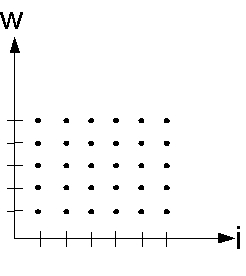
\includegraphics[scale=0.3]{\GRAPHPATH/psoas.jpg}
   \end{center}
\end{itemize}
}

\subsection{Intensions as functions}

\frame{\frametitle{The nature of propositions}
\begin{itemize}
  \item<1-> \gr{propositions = intensions of sentences (formulas)}
  \item<2-> remember the condition: every possible truth-value configuration for the full set of possible sentences constitutes a member of the set of possible worlds
  \item<3-> hence: every sentence is characterized by the set of worlds in which it is true
  \item<4-> this characterization: its intension
  \item<5-> \bl{the proposition of a sentence/formula: the characteristic function of the set of world/world-time pairs in which it is true}
\end{itemize}
}

\frame{\frametitle{Propositions as functions}
\begin{itemize}
  \item<1-> a propositional function $p$
  \item<2-> is a function from $W\times I$ to $\{0,1\}$\\
  
  \medskip
   \begin{center}
     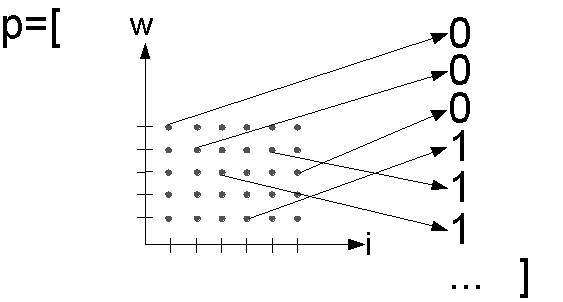
\includegraphics[scale=0.3]{\GRAPHPATH/propfunction.jpg}
   \end{center}
\end{itemize}
}

\subsection{Repeat after me...}
\frame{\frametitle{Your evening prayer}
\begin{itemize}
  \item<1-> \bl{If we know the state of affairs, we know for every sentence whether it is true!}
  \item<2-> \bl{If we know which sentences are true, we know the state of affairs!}
  \item<3-> It is quite difficult to state what other kind of knowledge (or information) should exist. So for now we assume there isn't any.
  \item<4-> Since we agree that sentences denote truth values, and that the truth of a sentence depends on the state of affairs (=world), \bl{the function from all possible worlds to truth values characterizes sentences under all thinkable conditions}.
  \item<5-> \bl{Hence, we call that function the intension of the sentence.}
\end{itemize}
}

\section{Sets of worlds}
\subsection{Known relations}

\frame{\frametitle{Entailment}
\begin{itemize}
  \item<1-> defintion of intensions of sentences (propositions): characteristic functions
  \item<2-> \bl{equivalently: propositions are sets of possible worlds}
  \item<3-> \bl{entailment} turns out as a \bl{subset-relation}: $p\subseteq q$:\\
  
  \medskip
   \begin{center}
     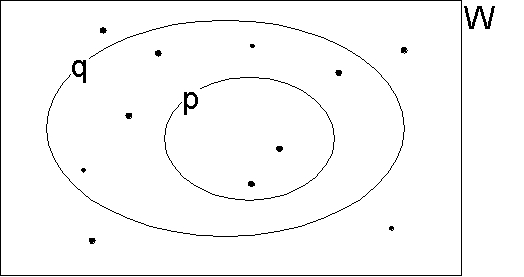
\includegraphics[scale=0.3]{\GRAPHPATH/entailment.jpg}
   \end{center}
\end{itemize}
}

\frame{\frametitle{Synonymy}
\begin{itemize}
  \item<1->\bl{synonymy} turns out as \bl{set equivalence}:\\
  \item<2-> $p=q$
  
  \medskip
   \begin{center}
     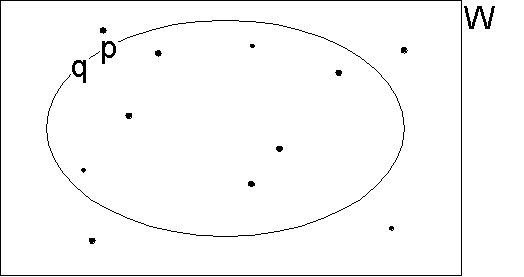
\includegraphics[scale=0.3]{\GRAPHPATH/equivalence.jpg}
   \end{center}
\end{itemize}
}

\frame{\frametitle{Contradiction}
\begin{itemize}
  \item<1->\bl{contradiction} turns out as an \bl{empty intersection}:\\
  \item<2-> $p\cap q=\emptyset$
  
  \medskip
   \begin{center}
     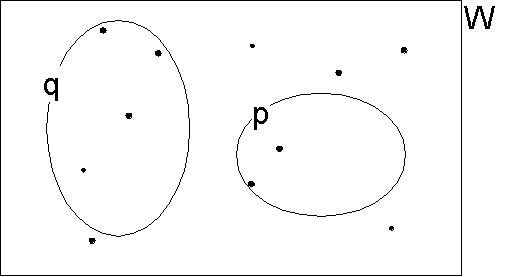
\includegraphics[scale=0.3]{\GRAPHPATH/contradiction.jpg}
   \end{center}
\end{itemize}
}

\frame{\frametitle{Negation}
\begin{itemize}
  \item<1->\bl{negation} turns out as a \bl{complement}:\\
  \item<2-> $p/W$
  
  \medskip
   \begin{center}
     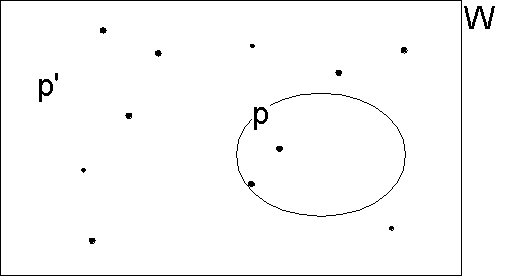
\includegraphics[scale=0.3]{\GRAPHPATH/not-p.jpg}
   \end{center}
\end{itemize}
}

\subsection{Modal operators}

\frame{\frametitle{Quantification over worlds}
\begin{itemize}
  \item<1-> new \bl{modal} sentence/wff operators:
    \begin{itemize}
      \item<2-> \emph{necessarily p}: \bl{$\mathbf{\Box{}p}$}
      \item<3-> \emph{possibly p}: \bl{$\mathbf{\Diamond{}p}$}
    \end{itemize}
  \item<4-> What does it mean for a proposition to be necessary/possible?
\end{itemize}
}

\frame{\frametitle{Necessity as universal quantification}
\begin{itemize}
  \item<1-> \bl{if $\Box{}p$ then $(\forall{}w)\ekm{p(w)=1}$} ($p$ as characteristic function)
  \item<2-> such that $W=p$ ($p$ as set):\\

  \medskip
   \begin{center}
     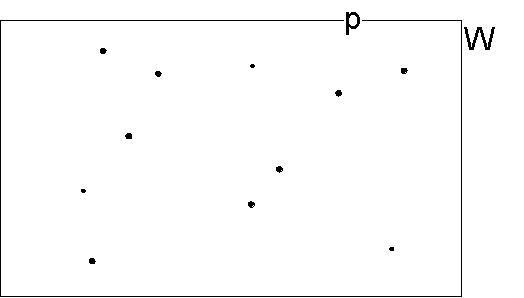
\includegraphics[scale=0.3]{\GRAPHPATH/necessarily-p.jpg}
   \end{center}\end{itemize}
}

\frame{\frametitle{Possibility as existential quantification}
\begin{itemize}
  \item<1-> \bl{if $\Diamond{}p$ then $(\exists{}w)\ekm{p(w)=1}$} (characteristic function)
  \item<2-> such that $p\not =\emptyset$ (set):\\

  \medskip
   \begin{center}
     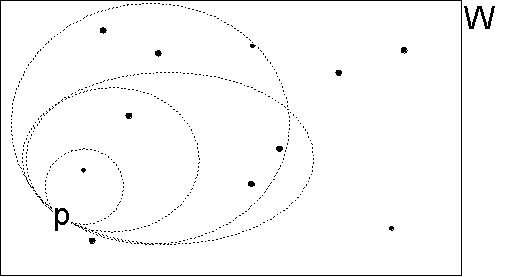
\includegraphics[scale=0.3]{\GRAPHPATH/possibly-p.jpg}
   \end{center}
\end{itemize}
}

\section{Intensional Model Theory}
\subsection{Ingedients of models}

\frame{\frametitle{A larger tuple}
\begin{itemize}
  \item<1->\bl{\Large $\mMm=\{W,I,<,U,V\}$}
    \begin{itemize}
      \item<2->$W$, a set of worlds
      \item<3->$I$, a set of instants
      \item<4->$<$, an ordering relation in I
      \item<5->$U$, the set of individuals
      \item<6->$V$, a valuation function for constants
    \end{itemize}
  \item<7-> \bl{evaluate an expression $\alpha$: $\DEMM{\alpha}$  }
\end{itemize}
}

\subsection{Evaluating individual constants}

\frame{\frametitle{Intensional interpretation of individual constants}
\begin{itemize}
  \item<1->\emph{the President of the United States}, \emph{the Pope}, \emph{Bond} (in the sense of `the actor currently playing Bond')
  \item<2->\bl{$for\ \beta\in Cons_{ind}, V(\beta)$ is a function from $W\times I$ to $U$}\\


  \medskip
   \begin{center}
     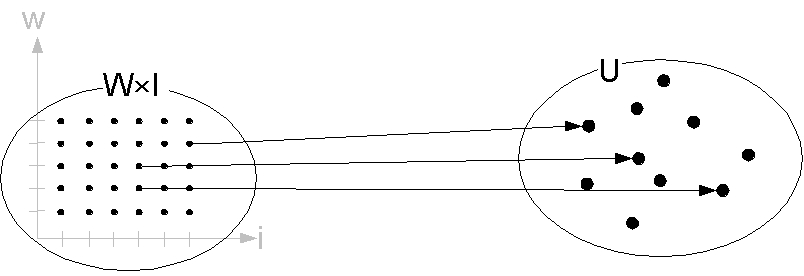
\includegraphics[scale=0.3]{\GRAPHPATH/wxi-to-u.jpg}
   \end{center}
\end{itemize}
}

\frame{\frametitle{... and pred\Sub{n}s}
\begin{itemize}
  \item<1->\emph{walks} etc. denotes different sets (or CFs) at different $\ram{w,i}$ coordinates
  \item<2->\bl{$for\ \beta\in Cons_{pred_n}, V(\beta)$ is a function from $W\times I$ to $\wp U^n\ (U^n=U_1\times U_2\times\ldots\times U_n)$}\\


  \medskip
   \begin{center}
     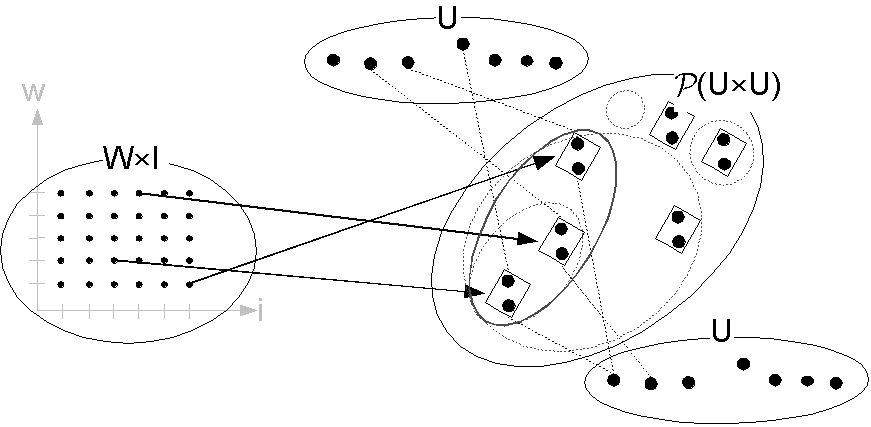
\includegraphics[scale=0.27]{\GRAPHPATH/wxi-to-Puxu.jpg}
   \end{center}
\end{itemize}
}

\subsection{Set membership}

\frame{\frametitle{The Chierchia approach: predicates/sentences}
\begin{itemize}
  \item<1-> simple sentences/predicates: \bl{$\beta=\delta(t_1,t_2,\ldots,t_n)$}
  \item<2->\bl{ $\DEMM{\beta}=1$} iff
  \item<3-> \bl{$\ram{\DEMM{t_1},\DEMM{t_2},\ldots,\DEMM{t_n}}\in\DEMM{\delta}$}
  \item<4-> with: $\DEMM{t_1}=V(t_1)(\ram{w,i})$, etc.
  \item<5-> \gr{In an intensional type-theoretic language, we could define new functional types and try to use FA where possible.}
\end{itemize}
}

\frame{\frametitle{Quantification}
\begin{itemize}
  \item<1-> if $\psi=\forall x\phi$ then
  \item<2-> \ldots $\DEMM{\psi}=1$ iff for all $u\in U$
  \item<3-> \ldots $\Dem{\phi}{\mMm,w,i,g[u/x]}=1$
  \item<4-> \gr{nothing new here}
\end{itemize}
}

\frame{\frametitle{Modalities}
\begin{itemize}
  \item<1-> if $\psi=\Box x\phi$ then
  \item<2-> \ldots $\DEMM{\psi}=1$ iff for all $w^{\prime}\in W$
  \item<3-> \gr{\ldots and all $i^{\prime}\in I$}
  \item<4-> \ldots $\Dem{\phi}{\mMm,w^{\prime},i^{\prime},g}=1$
\end{itemize}
}

\subsection{Some peculiarities of $\Box$ and $\Diamond$}

\frame{\frametitle{A similarity of $\forall$ and $\Box$}
\begin{itemize}
  \item<1-> as: $\forall x\ekm{P(x)\rightarrow Q(x)} \mathbf{\rightarrow} \ekm{\forall xP(x) \rightarrow \forall x Q(x)}$
  \item<2-> and not vice-versa
  \item<3-> it holds that: \bl{$\Box\ekm{\psi\rightarrow\phi}\rightarrow\ekm{\Box \psi\rightarrow\Box\phi}$}
  \item<4-> \rot{but not vice-versa!}
\end{itemize}
}

\frame{\frametitle{Some validities}
\begin{itemize}
  \item<1-> $\exists x\Box P(x)\rightarrow\Box\exists x P(x)$
  \item<2-> $\exists x\Diamond P(x)\leftrightarrow\Diamond\exists x P(x)$
  \item<3-> $\forall x\Box P(x)\leftrightarrow\Box\forall x P(x)$ (Carnap-Barcan)
  \item<4-> $\forall x\Diamond P(x)\rightarrow\Diamond\forall x P(x)$
\end{itemize}
}

